\chapter{赋值除环上的拓扑向量空间}

\section{拓扑向量空间}

\subsection{拓扑向量空间的定义}

定义 1. --- 给定一个拓扑除环 K (GT, III, § 6.7) 和一个集合 E，使得 E 具有

\(1^{\circ}\) \(\mathbf{K}\) 上的左向量空间结构；

\(2^{\mathrm{o}}\) 一个与 E 的加法群结构相容的拓扑 (GT, III,

§ 1.1)，且此外还满足下面的公理：

(EVT) 映射 \((\lambda, x) \mapsto \lambda x\)（\(\mathbf{K} \times \mathbf{E}\) 到 \(\mathbf{E}\) 中的映射）连续，

则称 E 为 K 上的左拓扑向量空间。

这等价于说 E 是一个拓扑左 K-模 (GT, III, § 6.6)。

集合 E 上相对于 K 的左向量空间结构与 E 上给定的拓扑称为相容的，如果该拓扑与 E 的加法群结构相容，并且此外公理 (EVT) 成立。这也就是说，\((x, y) \mapsto x + y\) 与 \((\lambda, x) \mapsto \lambda x\) 这两个映射（分别为 \(E \times E\) 与 \(K \times E\) 到 E 中的映射）都连续；因为这时映射 \(x \mapsto -x = (-1)x\) 连续，从而 E 的拓扑与其加法群结构相容。

若 \(\mathbf{E}\) 是 \(\mathbf{K}\) 上的左拓扑向量空间，则我们称仅赋有向量空间结构的 \(\mathbf{E}\) 是拓扑向量空间 \(\mathbf{E}\) 的底空间。

与 R 上 E 的向量空间结构相容。因为，设 \(u_{0}\) 为 E 中一点，设 H 为 X 的紧子集，并设 \(\varepsilon\) 为任意一个严格正的数。实值函数 \(u_{0}\) 在 H 上有界；令 \(a = \sup_{t \in H} |u_{0}(t)|\)；若 u 是 E 的任意一点，则对一切 \(t \in H\)

\[
\left| \lambda u (t) - \lambda_ {0} u _ {0} (t) \right| \leqslant | \lambda |. \left| u (t) - u _ {0} (t) \right| + a \left| \lambda - \lambda_ {0} \right|.
\]

于是，若 \(|\lambda - \lambda_0| \leqslant \varepsilon\) 且 \(|u(t) - u_0(t)| \leqslant \varepsilon\) 对一切 \(t \in \mathbf{H}\) 成立，则对 \(t \in \mathbf{H}\) 有 \(|\lambda u(t) - \lambda_0 u_0(t)| \leqslant \varepsilon (\varepsilon + |\lambda_0| + a)\)，这表明公理 (EVT) 得到满足；同样可以验证，紧收敛拓扑与 \(\mathbf{E}\) 的加法群结构相容。

另一方面，若 X 不是紧的，（X 上的）一致收敛拓扑未必与 E 的向量空间结构相容；例如，若 X = R 且 \(u_{0}\) 是 R 上的一个无界连续函数，则 R 到 E 中的映射 \(\lambda \mapsto \lambda u_{0}\) 在 E 的一致收敛拓扑下不连续。

\begin{enumerate}
\def\labelenumi{\arabic{enumi})}
\setcounter{enumi}{4}
\tightlist
\item
  设 E 是拓扑除环 K 上有限维 n 的向量空间；存在一个向量 K-空间的同构 \(u:K_{s}^{n}\to E\)，而且，若 v 是 \(K_{s}^{n}\) 到 E 上的第二个同构，则可以写 \(v=u\circ f\)，其中 f 是向量 K-空间 \(K_{s}^{n}\) 的一个自同构。在 \(K_{s}^{n}\) 上考虑与其向量空间结构相容的乘积拓扑（例 3）；由于 \(K_{s}^{n}\) 到自身的每个线性映射对该拓扑都连续，故向量空间 \(K_{s}^{n}\) 的每个自同构都是双连续的。因此，若借助 \(K_{s}^{n}\) 到 E 上的随便哪一个同构，把 \(K_{s}^{n}\) 的乘积拓扑搬到 E 上，则如此在 E 上得到的拓扑与所用的是哪个同构无关；我们称之为 E 上的典范拓扑；当 K 是一个非离散的完备赋值除环时，我们将另行刻画它 (I, § 1.3)。对于 E 上的典范拓扑，E 到 K 上任一拓扑向量空间中的每个线性映射都连续。
\end{enumerate}

按照与定义 1 相同的方式，可以定义拓扑除环 K 上的右拓扑向量空间；但 K 上的每个右向量空间都可以看作 K 的反除环 \(K^{0}\) 上的左向量空间 (A, II, § 1.1)，而且 K 的拓扑与除环 \(K^{0}\) 的结构相容。由于这个原因，我们通常只考虑左拓扑向量空间；当我们不带限定地说“拓扑向量空间”时，应理解为指的是左向量空间。

若 \(K'\) 是 K 的子除环，而 E 是 K 上的拓扑向量空间，则显然 E 的拓扑仍然与把标量域限制到 \(K'\) 后 E 相对于 \(K'\) 的向量空间结构相容；我们说按此程序得到的 \(K'\) 上的拓扑向量空间是 K 上拓扑向量空间 E 的底空间。

为使拓扑向量空间 E 是 Hausdorff 的，必须且只需：对 E 中每个 \(x \neq 0\)，存在一个不含 x 的 0 的邻域 (GT, III, § 1.2)。

在拓扑除环 K 上的向量空间 E 上，考虑一个与其加法群结构相容的拓扑。由于恒等式

\[
\lambda x - \lambda_ {0} x _ {0} = (\lambda - \lambda_ {0}) x _ {0} + \lambda_ {0} (x - x _ {0}) + (\lambda - \lambda_ {0}) (x - x _ {0})
\]

公理 (EVT) 等价于由下面三条公理组成的公理组。

(EVT') 对所有 \(x_0 \in \mathrm{E}\)，映射 \(\lambda \mapsto \lambda x_0\) 在 \(\lambda = 0\) 处连续。

(EVT \(_{II}\) ) 对所有 \(\lambda_{0}\in K\)，映射 \(x\mapsto\lambda_{0}x\) 在 x=0 处连续。

\((\mathrm{EVT}_{\mathrm{III}}^{\prime})\) 映射 \((\lambda, x) \mapsto \lambda x\) 在 \((0, 0)\) 处连续。

特别地：

命题 1. --- 对所有 \(\alpha \in \mathbf{K}\) 及每一点 \(b \in \mathbf{E}\)，映射 \(x \mapsto \alpha x + b\)（\(\mathbf{E}\) 到自身的映射）连续。此外，若 \(\alpha \neq 0\)，则该映射是 \(\mathbf{E}\) 到自身的一个同胚。

命题的第二部分来自如下事实：若 \(\alpha \neq 0\)，则 \(x \mapsto \alpha^{-1}x - \alpha^{-1}b\) 是 \(x \mapsto \alpha x + b\) 的逆映射。

推论. --- 若 A 是 E 中的开集（相应地，闭集），则 \(\alpha A\) 对 K 中每个 \(\alpha \neq 0\) 都是 E 中的开集（相应地，闭集）。

设 E 和 F 是同一拓扑除环 K 上的两个拓扑向量空间。E 到 F 上的双射 f 是拓扑向量空间 E 到拓扑向量空间 F 的同构，当且仅当 f 是线性的且双连续。特别地，若 \(\gamma \neq 0\) 属于 K 的中心，则位似 \(x \mapsto \gamma x\) 是 E 的拓扑向量空间结构的一个自同构。

\subsection{赋值除环上的赋范空间}

回忆 (GT, IX, § 3.2)，除环 K 上的绝对值是一个映射 \(\xi \mapsto |\xi|\)（K 到 \(\mathbf{R}_{+}\) 中的映射），使得 \(|\xi| = 0\) 当且仅当 \(\xi = 0\)，并且 \(|\xi \eta| = |\xi| \cdot |\eta|\)，以及 \(|\xi + \eta| \leqslant |\xi| + |\eta|\)；绝对值在 K 上定义了一个距离 \(|\xi - \eta|\)，从而定义了一个与 K 的除环结构相容的 Hausdorff 拓扑。若 \(|\xi| = 1\) 对所有 \(\xi \neq 0\) 成立，则称该绝对值为非真绝对值，它在 K 上定义的拓扑是离散拓扑；反之，若存在 K 中的 \(\alpha \neq 0\) 使 \(|\alpha| \neq 1\)，则存在 K 中的 \(\beta \neq 0\) 使 \(|\beta| < 1\)（只需取 \(\beta = \alpha\) 或 \(\beta = \alpha^{-1}\)），并且序列 \((\beta^n)_{n \geqslant 1}\) 收敛于 0，从而 K 的拓扑不是离散的。

另一方面我们回忆 (GT, IX, § 3.3)，若 E 是非离散赋值除环 K 上的向量空间，则 E 上的范数是一个映射 \(x \mapsto \|x\|\)（E 到 \(\mathbf{R}_{+}\) 中的映射），使得 \(\|x\| = 0\) 当且仅当 \(x = 0\)，并且 \(\| \lambda x \| = |\lambda| \cdot \| x\|\) 对每个标量 \(\lambda \in \mathbf{K}\) 成立，以及 \(\|x + y\| \leqslant \|x\| + \|y\|\)。范数在 E 上定义了一个距离 \(\|x - y\|\)，从而定义了一个与 E 的向量空间结构相容的拓扑 (loc. cit.)。除非另有明确说明，赋范空间总是就其范数所定义的拓扑向量空间结构来考虑。赋范空间属于最重要的拓扑向量空间之列。

我们知道 (GT, IX, § 3.3)，E 上两个不同的范数可以在 E 上定义同一个拓扑；为此必须且只需这两个范数等价 (loc. cit.)。因此赋范空间的结构比拓扑向量空间的结构更为丰富；若 E 和 F 是两个赋范空间，就必须注意区分 E 的赋范空间结构与 F 的赋范空间结构之间的同构概念，以及 E 的拓扑向量空间结构与 F 的拓扑向量空间结构之间的同构概念。

例. --- 设 I 为任意指标集；我们知道 (GT, X, § 3.2)，一个范数 \(\|x\|\) 可以定义在 I 到 K 中的有界映射 \(x = (\xi_{\mathfrak{t}})\) 所成的集合 \(\mathcal{B}(\mathrm{I};\mathrm{K})\)（也记作 \(\mathcal{B}_{\mathrm{K}}(\mathrm{I})\) 或 \(\ell_{\mathrm{K}}^{\infty}(\mathrm{I})\)）上，其定义为 \(\|x\| = \sup_{\mathfrak{t}\in \mathrm{I}}|\xi_{\mathfrak{t}}|\)。当 I 是拓扑空间时，I 到 K 中的有界连续映射所成的集合是空间 \(\mathcal{B}(\mathrm{I};\mathrm{K})\) 的闭子空间 (GT, X, § 3.1, cor. 2)。\(\mathcal{B}(\mathrm{I};\mathrm{K})\) 的另一个子空间是 \(\ell_{\mathrm{K}}^{1}(\mathrm{I})\)，即绝对可和族 \(x = (\xi_{\mathfrak{t}})\) 所成的集合 (GT, X, § 3.6)；在这个子空间上可以定义另一个范数 \(\|x\|_1 = \sum_{\mathfrak{t}\in \mathrm{I}}|\xi_{\mathfrak{t}}|\)，它一般与范数 \(\|x\| = \sup_{\mathfrak{t}\in \mathrm{I}}|\xi_{\mathfrak{t}}|\) 不等价 (I, 第 23 页, 习题 6)；当把 \(\ell_{\mathrm{K}}^{1}(\mathrm{I})\) 视为赋范空间而不指明其范数时，所指的总是范数 \(\|x\|\)。我们用 \(\mathcal{B}(\mathrm{I})\) 与 \(\ell^1 (\mathrm{I})\) 代替 \(\mathcal{B}(\mathrm{I};\mathbf{R})\) 与 \(\ell_{\mathbf{R}}^{1}(\mathrm{I})\)。

\subsection{拓扑向量空间的向量子空间与商空间；拓扑向量空间的乘积；子空间的拓扑直和}

对拓扑模块 (GT, III, § 6.6) 所说的一切特别适用于拓扑向量空间。若 M 是拓扑向量空间 E 的向量子空间，则由 E 的拓扑在 M 上诱导的拓扑与 M 的向量空间结构相容，并且 M 在 E 中的闭包 \(\overline{M}\) 是 E 的向量子空间。E 的拓扑对 M 的商拓扑与 E/M 的向量空间结构相容。

若 E 是拓扑向量空间，则 \(\{0\}\) 在 E 中的闭包 N（0 的各邻域之交）是 E 的闭向量子空间；商向量空间 E/N 必定是 Hausdorff 的（不论 E 本身是否如此），称为与 E 相伴的 Hausdorff 向量空间。

设 \((\mathrm{E}_{\iota})_{\iota \in I}\) 是同一拓扑除环 K 上的一族拓扑向量空间，并设 E 是诸 \(E_{\iota}\) 的乘积向量空间。诸 \(E_{\iota}\) 的拓扑的乘积拓扑与 E 的向量空间结构相容。在乘积空间 E 中，诸 \(E_{\iota}\) 的直和所构成的子空间 F 处处稠密 (GT, III, § 2.9, prop. 25)。

对 \(\mathbf{R}\) 域或 \(\mathbf{C}\) 域上某些类型的拓扑向量空间，我们 (在 II, 第 29 页) 在一族拓扑向量空间 \((\mathrm{E}_{\mathrm{t}})\) 的直和上定义一个拓扑，它一般不同于由诸 \(\mathrm{E}_{\mathrm{t}}\) 的乘积拓扑所诱导的拓扑。

关于带算子的拓扑群的稳定子群的有限直和所说的一切 (GT, III, §6.2) 都适用于拓扑向量空间，只需把其中的“稳定子群”一律换成“向量子空间”。

注记. --- 给定 Hausdorff 拓扑向量空间 E 的闭向量子空间 M，未必存在 M 在 E 中的（代数）补向量子空间在 E 中闭（即使 E 是赋范空间亦然；参见 IV, 第 55 页, 习题 16 (c)）；更谈不上 M 在 E 中的拓扑补必定存在 (参见 I, 第 26 页, 习题 8)。然而我们将在 § 2 中看到，当 K 是非离散赋值除环时，E 的每个具有有限余维数的闭子空间 M 在 E 中确实有拓扑补 (I, 第 14 页, prop. 3)。

\subsection{拓扑向量空间的一致结构与完备化}

由于拓扑向量空间 E 的拓扑与 E 上的加法群结构相容，它在 E 上定义了一个一致结构 (GT, III, § 3)；当我们谈到拓扑向量空间的一致结构时，除非另有明确说明，指的总是这个结构。拓扑向量空间 E 到拓扑向量空间 F 中的每个连续线性映射都是一致连续的 (GT, III, § 3.1, prop. 3)；E 到自身中每个形如 \(x \mapsto ax + b\) 的映射都是一致连续的。E 到 F 中的线性映射的一个等度连续集是一致等度连续的 (GT, X, § 2.2, prop. 5)。

注记. --- 1) 若 B 是 K 的预紧集，则对 E 中 0 的每个邻域 V，存在 E 中 0 的一个邻域 U，使得 BU ⊂ V。因为，若 W 是 E 中 0 的一个邻域使得 W + W ⊂ V，则由 (EVT \(_{III}\) )，存在 K 中 0 的一个邻域 T \(_{0}\) 和 E 中 0 的一个邻域 U \(_{0}\)，使得 T \(_{0}\) U \(_{0}\) ⊂ W。由于 B 是预紧的，存在有限多个点 \(\lambda_{i} \in \mathbf{B}\) ( \(1 \leqslant i \leqslant n\) ) 使诸 \(\lambda_{i} + T_{0}\) 覆盖 B；由 (EVT \(_{II}\) ) 推出，存在 E 中 0 的一个邻域 U ⊂ U \(_{0}\)，使对所有 i 有 \(\lambda_{i}\) U ⊂ W；显然 U 具有所需的性质。类似地（用 (EVT \(_{I}\) ) 代替 (EVT \(_{II}\) )）可以证明：若 H 是 E 的预紧集，则对 E 中 0 的每个邻域 V，存在 K 中 0 的一个邻域 T，使得 TH ⊂ V。

\begin{enumerate}
\def\labelenumi{\arabic{enumi})}
\setcounter{enumi}{1}
\tightlist
\item
  由 1) 推出，若 B 是 K 的预紧集而 H 是 E 的预紧集，则映射 \((\lambda, x) \mapsto \lambda x\) 限制在 \(\mathbf{B} \times \mathbf{H}\) 上是一致连续的。因为，若 V 是 E 中 0 的一个邻域，则存在 K 中 0 的邻域 T 和 E 中 0 的邻域 U，使得 \(\mathrm{TH} + \mathrm{BU} \subset \mathrm{V}\)。由于可以写 \(\lambda x - \lambda' x' = (\lambda - \lambda') x + \lambda'(x - x')\)，我们看到，当 \(\lambda, \lambda'\) 属于 B，\(x, x'\) 属于 H，且 \(\lambda - \lambda' \in \mathrm{T}\) 及 \(x - x' \in \mathrm{U}\) 时，有 \(\lambda x - \lambda' x' \in \mathrm{V}\)，这就证明了我们的断言。
\end{enumerate}

拓扑向量空间称为完备的，如果就其一致结构考虑，它是一个完备一致空间。

定义 2. --- 非离散赋值除环上的完备赋范空间称为 Banach 空间。

例. --- 若 K 是非离散赋值除环，则空间 \(\mathcal{B}(\mathrm{I};\mathrm{K})\) (I, 第 4 页, 例) 是完备的 (GT, X, § 3.1, cor. 1)。对于空间 \(\ell_{\mathbf{K}}^{1}(\mathrm{I})\) (I, 第 4 页, 例)，带范数 \(\| x\| _1 = \sum_{\iota \in \mathrm{I}}|\xi_\iota |:\) 情形也是如此：因为，若 \(x_{n}\) 是该空间中的一个 Cauchy 序列且 \(x_{n} = (\xi_{n\iota})_{\iota \in \mathrm{I}}\)，则对所有 \(\iota \in \mathrm{I}\)

\[
\left| \xi_ {m\iota} - \xi_ {n\iota} \right| \leqslant \left\| x _ {m} - x _ {n} \right\| _ {1};
\]

于是，对每个 \(\iota \in I\)，序列 \((\xi_{n\iota})_{n\geqslant 1}\) 在 K 中收敛于一个极限 \(\xi_{\iota}\)。此外，对 I 的每个有限子集 J

\[
\sum_ {\iota \in J} | \xi_ {m\iota} - \xi_ {n\iota} | \leqslant \| x _ {m} - x _ {n} \| _ {1};
\]

由此立即推出，存在一个常数 \(a > 0\)（与 J、\(m, n\) 无关），使得 \(\sum_{\iota \in \mathbf{J}} |\xi_{m\iota} - \xi_{n\iota}| \leqslant a\)。令 \(m\) 趋于 \(+\infty\)，我们推出 \(\sum_{\iota \in \mathbf{J}} |\xi_{\iota} - \xi_{n\iota}| \leqslant a\)，由此得 \(\sum_{\iota \in \mathbf{I}} |\xi_{\iota}| \leqslant a + \| x_n\|_1\)，这表明 \(z = (\xi_{\iota})_{\iota \in \mathbf{I}}\) 属于 \(\ell_{\mathbf{K}}^1 (\mathbf{I})\)；此外，对所有 \(\varepsilon > 0\)，存在 \(n_0\)，使得当 \(n \geqslant n_0\) 且 J 为 I 的任意有限子集时，有 \(\sum_{\iota \in \mathbf{J}} |\xi_{\iota} - \xi_{n\iota}| \leqslant \varepsilon\)；关于 I 的有限子集所成的定向集取极限，我们看出 \(\| z - x_n\| _1\leqslant \varepsilon\) 对 \(n\geqslant n_0\) 成立，这表明 \(z\) 是序列 \((x_{n})\) 在赋范空间 \(\ell_{\mathbf{K}}^{1}(\mathrm{I})\) 中的极限

设 K 是 Hausdorff 拓扑除环，E 是 K 上的拓扑向量空间，并设完备化环 \(\hat{K}\) 是一个除环（当 K 是赋值除环时即是如此，GT, IX, § 3.3），则 E 的分离完备化 \(\hat{E}\) 具有 \(\hat{K}\) 上完备拓扑向量空间的结构 (GT, III, § 6.5)；我们说带有这一结构的 \(\hat{E}\) 是拓扑向量空间 E 的分离完备化，而当 E 是 Hausdorff 时简称其为 E 的完备化。

\subsection{赋值除环上的拓扑向量空间中原点的邻域}

定义 3. --- 设 K 是赋值除环，E 是 K 上的左向量空间；我们称 E 的子集 M 是均衡的，如果对所有 \(x \in M\) 及所有 \(\lambda \in K\)，只要 \(|\lambda| \leqslant 1\)，就有 \(\lambda x \in M\)（换言之，如果 \(\lambda M \subset M\) 只要 \(|\lambda| \leqslant 1\)）。

命题 2. --- 在赋值除环 K 上的拓扑向量空间 E 中，均衡集 M 的闭包是均衡集。

若 B 是由 \(\xi\in K\)（满足 \(|\xi|\leqslant1\)）组成的集，则 B 在 K 中闭。而 \(B\times M\) 被连续映射 \((\lambda,x)\mapsto\lambda x\) 映入 M；因此 \(B\times\overline{M}\) 被映入 \(\overline{M}\) (GT, I, §2.1, th. 1)，这就证明 \(\overline{M}\) 是均衡的。

当 M 是赋值除环 K 上的向量空间 E 中的任意集合时，集合 \(M_{1}\)（即诸 \(\lambda x\)，其中 \(x \in M\)、\(\lambda \in K\) 且 \(|\lambda| \leqslant 1\)）显然是包含 M 的最小均衡集；\(M_{1}\) 称为 M 的均衡包。

命题 3. --- 设 K 是局部紧的非离散赋值除环，E 是 K 上的 Hausdorff 拓扑向量空间（相应地，拓扑向量空间）。对 E 中每个紧（相应地，预紧）集 H，H 的均衡包是紧的（相应地，预紧的）。

若 B 表示 K 中的球 \(|\xi| \leqslant 1\)，则 H 的均衡包就是 \(H_{1}\)，即 \(B \times H\) 在连续映射 \(m: (\lambda, x) \mapsto \lambda x\) 下的像。若 E 是 Hausdorff 的，B 与 H 都是紧的，则 \(B \times H\) 从而 \(H_{1}\) 也是紧的。若 H 是预紧的，则 m 在 \(B \times H\) 上的限制是一致连续的 (I, 第 5 页, 注记 2)，而由于 \(B \times H\) 预紧，其在 m 下的像也是预紧的 (GT, II, § 4.2, prop. 2)。

注意，闭集的均衡包未必闭。例如在 \(\mathbf{R}^2\) 中，由方程 \(xy = 1\) 定义的双曲线的均衡包不是闭的。

E 中一族均衡集的并是均衡的，由此推出，对 E 的每个集合 M，存在包含在 M 中的最大均衡子集 N，称为 M 的均衡核；而且 N 非空当且仅当 \(0 \in M\)。说 \(x \in N\) 意味着对所有 \(\lambda \in K\)，只要 \(|\lambda| \leqslant 1\)，就有 \(\lambda x \in M\)，或者（当 \(0 \in M\) 时）等价地，对所有 \(\mu \in K\)，只要 \(|\mu| \geqslant 1\)，就有 \(x \in \mu M\)。若 \(0 \in M\)，则 M 的均衡核 N 就是交集 \(\bigcap_{|\mu| \geqslant 1} \mu M\)。这特别表明，若 M 闭，则 N 也闭。

定义 4. --- 设 K 是非离散赋值除环，E 是 K 上的左向量空间且带有两个子集 A 和 B。我们称 A 吸收 B，如果存在 \(\alpha > 0\)，使得 \(\lambda A \supset B\) 对每个 \(\lambda \in K\) 只要 \(|\lambda| \geqslant \alpha\) 就成立（等价地，如果 \(\mu B \subset A\) 对 \(\mu \neq 0\) 且 \(|\mu| \leqslant \alpha^{-1}\) 成立）。E 的集合 A 称为吸收集，如果它吸收每个由单独一点组成的集合。

设 A 是 E 的均衡集；为使 A 吸收 E 的集合 B，只需存在 \(\lambda \neq 0\) 使 \(\lambda A \supset B\)；事实上，当 \(|\mu| \geqslant |\lambda|\) 时，有 \(\lambda A = (\lambda \mu^{-1}) \mu A\)，而由于 \(\mu A\) 均衡且 \(|\lambda \mu^{-1}| \leqslant 1\)，由此推出 \(\lambda A \subset \mu A\)，从而 \(B \subset \mu A\)。特别地，为使 E 的均衡集 A 是吸收集，必须且只需：对每个 \(x \in E\)，存在 K 中的 \(\lambda \neq 0\) 使 \(\lambda x \in A\)。E 的每个吸收集生成向量空间 E。吸收集的每个有限交是吸收集。

命题 4. --- 在非离散赋值除环 K 上的拓扑向量空间 E 中，存在 0 的闭邻域组成的一个基本邻域系 \(\mathfrak{B}\)，使得：

\((\mathrm{EV}_{\mathrm{I}})\) 每个 \(\mathbf{V}\in \mathfrak{B}\) 都是均衡的且是吸收的。

(EV \(_{II}\) ) 对每个 V \(\in\) B 及 K 中的 \(\lambda \neq 0\)，有 \(\lambda\) V \(\in\) B（B 在比不为零的位似下不变）。

\((\mathrm{EV}_{\mathrm{III}})\) 对每个 \(\mathbf{V}\in \mathfrak{B}\)，存在 \(\mathbf{W}\in \mathfrak{B}\) 使得 \(\mathbf{W} + \mathbf{W}\subset \mathbf{V}\)。

反之，设 E 是 K 上的向量空间，V 是 E 上满足条件 \((\mathrm{EV}_{\mathrm{I}})\)、\((\mathrm{EV}_{\mathrm{II}})\) 与 \((\mathrm{EV}_{\mathrm{III}})\) 的一个滤子基。则在 E 上存在（且唯一）一个与 E 的向量空间结构相容的拓扑，使 V 构成 0 的一个基本邻域系。

由公理 \((\mathrm{EVT}_{\mathrm{III}}^{\prime})\)，我们首先证明：0 的邻域 V 的均衡核 \(V_{1}\) 本身是 0 的邻域。因为存在 \(\alpha > 0\) 及 0 的一个邻域 W，使得当 \(|\lambda| \leqslant \alpha\) 且 \(x \in W\) 时，有 \(\lambda x \in V\)。由于 K 非离散，存在 K 中的 \(\mu \neq 0\) 满足 \(|\mu| \leqslant \alpha\)，而 \(\mu W\) 是 0 的一个邻域且 \(\mu W \subset V\)。又若 \(v \in K\) 且 \(|v| \leqslant 1\)，则 \(|v\mu| \leqslant \alpha\)，从而 \(v\mu W \supset V\)。于是 \(\mu W \supset V_{1}\)，故 \(V_{1}\) 是 0 的邻域。又由于 V 闭，\(V_{1}\) 也闭。因此，0 的闭均衡邻域所成的集 B 构成 E 中 0 的一个基本邻域系。由 \((\mathrm{EVT}_{\mathrm{I}}^{\prime})\)，0 的每个邻域都是吸收的；此外 B 满足 \((\mathrm{EV}_{\mathrm{II}})\) (参见 I, 第 3 页, cor.)；最后，由于 \((x, y) \mapsto x + y\) 在点 \((0, 0)\) 处连续，E 中 0 的每个基本邻域系都满足 \((\mathrm{EV}_{\mathrm{III}})\)。于是集 B 满足命题中的条件。

现在设 E 是 K 上的向量空间，V 是 E 上满足 \((\mathrm{EV}_{\mathrm{I}})\)、\((\mathrm{EV}_{\mathrm{II}})\) 与 \((\mathrm{EV}_{\mathrm{III}})\) 的一个滤子基。公理 \((\mathrm{EV}_{\mathrm{I}})\) 首先表明，对所有 \(V \in V\)，有 -V = V 及 \(0 \in V\)；这些关系式与公理 \((\mathrm{EV}_{\mathrm{III}})\) 表明，V 构成 E 上与 E 的加法群结构相容的某个拓扑 (GT, III, § 1.2) 下 0 的基本邻域系。另一方面，公理 (EVT \(_{I}\) )、(EVT \(_{II}\) ) 与 (EVT \(_{III}\) ) 是 (EV \(_{I}\) ) 与 (EV \(_{II}\) ) 的直接推论，因此上面定义的拓扑满足公理 (EVT)，命题得证。

注记. --- 1) 在非离散赋值除环上的赋范空间中，以 0 为中心的全体开球（相应地，闭球）构成 0 的一个基本邻域系，它满足条件 \((\mathrm{EV}_{\mathrm{I}})\)、\((\mathrm{EV}_{\mathrm{II}})\) 与 \((\mathrm{EV}_{\mathrm{III}})\)。

\begin{enumerate}
\def\labelenumi{\arabic{enumi})}
\setcounter{enumi}{1}
\tightlist
\item
  当标量除环 \(\mathbf{K}\) 是 \(\mathbf{R}\) 域或 \(\mathbf{C}\) 域时，每个滤子基 \(\mathfrak{B}\)（在 \(\mathbf{E}\) 上）若只满足两条公理 \((\mathrm{EV}_{\mathbf{I}})\) 与 \((\mathrm{EV}_{\mathrm{III}})\)，则它是某个与 \(\mathbf{E}\) 的向量空间结构相容的拓扑下 0 的基本邻域系。事实上，只需证明：在这些条件下，对每个 \(\lambda \neq 0\)（在 \(\mathbf{K}\) 中）及每个 \(\mathrm{V} \in \mathfrak{B}\)，存在 \(\mathrm{W} \in \mathfrak{B}\) 使得 \(\lambda \mathrm{W} \subset \mathrm{V}\)。由 \((\mathrm{EV}_{\mathrm{III}})\)，存在 \(\mathrm{W}_{1} \in \mathfrak{B}\) 满足 \(2\mathrm{W}_{1} \subset \mathrm{V}\)，并且我们用归纳法推出，对每个正整数 \(n\)，存在 \(\mathrm{W}_{n} \in \mathfrak{B}\) 使得 \(2^{n}\mathrm{W}_{n} \subset \mathrm{V}\)。由于 \(\mathrm{V}\) 是均衡的，只要取 \(n\) 大到使 \(2^{n} = |2^{n}| > |\lambda|\)，则 \(\mathrm{W} = \mathrm{W}_{n}\) 就满足条件，此即所需。
\end{enumerate}

这个结果并非对每个非离散赋值除环 K 都成立，因为在这种除环中，对每个正整数 m 不再必有 \(|me| = m\)（\(e\) 表示除环的单位元；参见 I, 第 22 页, 习题 1）。

\begin{enumerate}
\def\labelenumi{\arabic{enumi})}
\setcounter{enumi}{2}
\tightlist
\item
  若 K 是离散除环，则条件 \((\mathrm{EVT}_{\mathrm{I}}^{\prime})\) 与 \((\mathrm{EVT}_{\mathrm{III}}^{\prime})\) 对 E 上的任何拓扑都成立。按命题 4 的方式论证，容易看出：若 E 是 K 上的拓扑向量空间，则存在 E 中 0 的闭邻域组成的一个基本邻域系 B，满足条件 \((\mathrm{EV}_{\mathrm{II}})\) 与 \((\mathrm{EV}_{\mathrm{III}})\)。反之，若 K 上向量空间 E 上的滤子基 B 使得 0 属于 B 的所有集合，且 \((\mathrm{EV}_{\mathrm{II}})\)、\((\mathrm{EV}_{\mathrm{III}})\) 成立，则 B 是与 E 的向量空间结构相容的某个拓扑下 0 的基本邻域系。
\end{enumerate}

\subsection{连续性与等度连续性判别准则}

设 \(\mathbf{E}\) 与 \(\mathbf{F}\) 是同一除环 \(\mathbf{K}\) 上的拓扑向量空间；为使线性映射 \(f\)（\(\mathbf{E}\) 到 \(\mathbf{F}\) 中的映射）连续，只需它在原点连续 (GT, III, § 2.8, prop. 23)。该命题可推广如下：

命题 5. --- 设 \(E_{i}(1 \leqslant i \leqslant n)\) 与 F 是非离散赋值域 K 上的拓扑向量空间。为使 \(\prod_{i=1}^{n} E_{i}\) 到 F 中的多重线性映射 f 连

续于乘积空间 \(\prod_{i=1}^{n} E_i\) 中，只需它在 \((0, 0, ..., 0)\) 处连续。

设 \((a_{1}, a_{2}, \ldots, a_{n})\) 是 \(\prod_{i=1}^{n} \mathrm{E}_{i}\) 的任意一点；我们必须证明，对每个邻域 \(W\)（0 在 \(F\) 中的邻域），存在邻域 \(\mathrm{V}_{i}\)（0 在 \(\mathrm{E}_{i}\) 中的邻域）( \(1 \leqslant i \leqslant n\) )，使得诸关系式 \(z_{i} \in V\) 蕴含

\[
f \left(a _ {1} + z _ {1}, a _ {2} + z _ {2}, \dots , a _ {n} + z _ {n}\right) - f \left(a _ {1}, a _ {2}, \dots , a _ {n}\right) \in \mathrm{W}.
\]

现在，我们可以写成

\[
f (a _ {1} + z _ {1}, \dots , a _ {n} + z _ {n}) - f (a _ {1}, \dots , a _ {n}) = \sum_ {\mathrm{H}} u _ {\mathrm{H}}
\]

其中 H 取遍 \(2^{n}-1\) 个子集（即整数集 \(\{1,2,\ldots,n\}\) 的除 \(\{1,2,\ldots,n\}\) 本身以外的子集），而 \(u_{\mathrm{H}}=f(y_{1},y_{2},\ldots,y_{n})\)，其中 \(y_{i}=a_{i}\) 若 \(i\in H\)，而 \(y_{i}=z_{i}\) 若 \(i\notin H\)。存在 \(2^{n}-1\) 个 F 中 0 的均衡邻域 \(W_{H}\)，使得 \(\sum_{H}W_{H}\subset W\)；另一方面，由假设 f 在 \((0,0,\ldots,0)\) 处连续，故在每个 \(E_{i}\) 中存在 0 的一个邻域 \(U_{i}\) \(0(1\leqslant i\leqslant n)\)，使得 n 个关系式 \(x_{i}\in U_{i}\) 蕴含 \(f(x_{1},\ldots,x_{n})\in\bigcap_{\mathrm{H}}\mathrm{W}_{\mathrm{H}}\)。由于 \(U_{i}\) 是吸收的，存在 K 中的 \(\lambda_{i}\neq0\) 使得 \(\lambda_{i}a_{i}\in U_{i}\)。设 \(\lambda\) 是 K 中对每个子集 H 都满足 \(|\lambda|\geqslant\prod_{i\in H}|\lambda_{i}|^{-1}\) 的元素；我们证明邻域 \(V_{i}=\lambda^{-n}U_{i}\) 满足所需条件。可以写 \(u_{\mathrm{H}}=\mu f(x_{1},\ldots,x_{n})\)，其中 \(x_{i}\in U_{i}\)（对 \(1\leqslant i\leqslant n\)），而 \(\mu=\lambda^{-np}(\prod_{i\in H}\lambda_{i}^{-1})\)，p 是 \(\{1,2,\ldots,n\}\) 中不属于 H 的整数个数。由上式得 \(|\mu|\leqslant1\)，从而有 \(u_{H}\in\mu W_{H}\subset W_{H}\)，因为 \(W_{H}\) 均衡。命题得证。

命题 6. --- 在与命题 5 相同的关于 \(E_{i}(1 \leqslant i \leqslant n)\) 与 F 的假设下，为使 \(\prod_{i=1}^{n} E_{i}\) 到 F 中的多重线性映射所成的集 E 等度连续，只需该集在 \((0, 0, \ldots, 0)\) 处等度连续。

因为，在命题 5 的证明中，可以取 \(\mathrm{U}_i\) ( \(1 \leqslant i \leqslant n\) ) 使得关系式 \(x_i \in \mathrm{U}_i\) ( \(1 \leqslant i \leqslant n\) ) 蕴含 \(f(x_1, \ldots, x_n) \in \bigcap_{\mathrm{H}} \mathrm{W}_{\mathrm{H}}\) 对每个映射 \(f \in \mathcal{E}\) 成立。

\subsection{向量空间的初始拓扑}

命题 7. --- 设 \((\mathrm{E}_{\mathfrak{t}})_{\mathfrak{t}\in\mathbf{I}}\) 是拓扑除环 K 上的一族拓扑向量空间。设 E 是 K 上的向量空间，且对每个 \(\mathfrak{t}\in I\)，设 \(f_{t}\) 是 E 到 \(E_{t}\) 中的线性映射。则 E 上使每个函数 \(f_{t}\) 连续的最粗拓扑是 E 上与 E 的向量空间结构相容的拓扑 T。此外，若对每个 \(x\in E\)，\(\phi(x)\) 表示点 \((f_{\mathfrak{t}}(x))\)（乘积空间 \(F=\prod_{\mathfrak{t}\in I}E_{\mathfrak{t}}\) 中的点），则拓扑 T 是 F 的子空间 \(\phi(\mathrm{E})\) 的拓扑在线性映射 \(\phi\) 下的逆像。

命题的最后一部分是 GT, I, § 4.1, prop. 3 的特例。于是命题由下面的引理得出。

引理. --- 设 M 与 N 是两个向量空间，g 是 M 到 N 中的线性映射。若 \(T_{0}\) 是与 N 的向量空间结构相容的拓扑，则 \(T_{0}\) 在 g 下的逆像与 M 的向量空间结构相容。

例如我们证明，\((\lambda, x) \mapsto \lambda x\) 在每一点 \((\lambda_{0}, x_{0})\)（\(K \times M\) 中的点）处连续。令令 \(y_{0} = g(x_{0})\)。M 中 0 的每个邻域都包含形如 \(g(U)\) 的邻域，其中 U 是 N 中 0 的邻域；由假设，存在 K 中 0 的一个邻域 V 及 N 中 0 的一个邻域 W，使得关系式 \(\lambda - \lambda_{0} \in V\) 与 \(y - y_{0} \in W\) 蕴含 \(\lambda y - \lambda_{0}y_{0} \in U\)。于是关系式 \(\lambda - \lambda_{0} \in V\)、\(x - x_{0} \in g(W)\) 蕴含 \(\lambda x - \lambda_{0}x_{0} \in g(U)\)。类似地可以证明 \((x, y) \mapsto x - y\) 在 \(M \times M\) 中连续。

对每个指标 \(\iota \in I\)，设 \(\mathfrak{B}_{\iota}\) 是 \(E_{\iota}\) 中 0 的一个基本邻域系。由拓扑 \(\mathcal{T}\) 的定义，该拓扑下 0 的邻域滤子由诸族 \(\overline{f}_{\iota}^{1}(\mathfrak{B}_{\iota})\) 中的集合之并生成；换言之，形如 \(\bigcap_{k} \overline{f}_{\iota_k}^{-1}(V_{\iota_k})\) 的集合构成 \(\mathcal{T}\) 下 0 的一个基本邻域系，其中 \((\iota_k)_{1 \leqslant k \leqslant n}\) 是 I 的任意有限指标序列，而对每个指标 \(k\)，\(V_{\iota_k}\) 是 \(\mathfrak{B}_{\iota_k}\) 中的任意集合。

推论 1. --- 设 G 是 K 上的拓扑向量空间。为使 G 到 E 中的映射所成的集 H 等度连续，必须且只需：对所有 \(\iota \in I\)，当 u 在 H 中变化时 \(f_{\iota} \circ u\) 所成的集等度连续。

这是 GT, X, § 2.2, prop. 3 的特例。

推论 2. --- 若诸空间 \(E_{t}\) 是 Hausdorff 的，则为使 \(\mathcal{T}\) 是 Hausdorff 的，必须且只需：对每个 \(x \neq 0\)（在 \(E\) 中），存在指标 \(t \in I\) 使 \(f_{t}(x) \neq 0\)。

因为这时 \(\phi(E)\) 是 Hausdorff 空间，而为使 \(\mathcal{T}\) 是 Hausdorff 的，显然必须且只需 \(\phi\) 是单射；注意这时可以把 \(E\)（带 \(\mathcal{T}\)）与子空间 \(\phi(E)\)（\(\prod_{i} E_{i}\) 的子空间）借助于映射 \(\phi\) 等同起来。

推论 3. --- 设诸 \(E_{t}\) 完备且 \(\phi(E)\) 在 \(F = \prod_{t \in I} E_{t}\) 中闭。则 E 在拓扑 T 下完备。

因为这时子空间 \(\phi(E)\)（\(F\) 的子空间）完备 (GT, II, § 3.4, prop. 8 与 § 3.5, prop. 10)，因此在逆像拓扑下 \(E\) 亦然 (GT, I, § 7.6, prop. 10 及 GT, II, § 3.1, prop. 4)。

* 例. --- 设 \(\mathcal{D}'(\mathbf{R})\) 是 \(\mathbf{R}\) 上的广义函数空间；设 \(p\) 是满足 \(1 \leqslant p \leqslant +\infty\) 的数，令 \(j: \mathrm{L}^p(\mathbf{R}) \to \mathcal{D}'(\mathbf{R})\) 为典范单射，它是连续的（当 \(\mathrm{L}^p(\mathbf{R})\) 赋以其赋范空间拓扑而 \(\mathcal{D}'(\mathbf{R})\) 赋以强拓扑时）。对每个广义函数 \(f \in \mathcal{D}'(\mathbf{R})\)，把 \(f\) 的导数记作 \(\mathrm{D}(f)\)；回忆 \(f \mapsto \mathrm{D}(f)\) 是 \(\mathcal{D}'(\mathbf{R})\) 的连续自同态。于是设 E 是 \(\mathrm{L}^p(\mathbf{R})\) 的向量子空间，由那些 \(f \in \mathrm{L}^p(\mathbf{R})\)（满足 \(\mathrm{D}(f) \in \mathrm{L}^p(\mathbf{R})\)）组成，并在 E 上赋予使典范单射 \(i: \mathrm{E} \to \mathrm{L}^p(\mathbf{R})\) 与映射 \(\mathrm{D}: \mathrm{E} \to \mathrm{L}^p(\mathbf{R})\) 都连续的最粗拓扑（\(\mathrm{L}^p(\mathbf{R})\) 赋以其赋范空间拓扑）。对这个拓扑，空间 E 是完备的。因为，E 在 \(\mathrm{F} = \mathrm{L}^p(\mathbf{R}) \times \mathrm{L}^p(\mathbf{R})\) 中经映射 \(\phi: f \mapsto (f, \mathrm{D}(f))\) 所成的像是闭的，因为它是像 G 在 \(\mathrm{L}^p(\mathbf{R}) \times \mathrm{L}^p(\mathbf{R})\) 上的迹，其中 G 是 \(\mathcal{D}'(\mathbf{R})\) 在 \(\mathcal{D}'(\mathbf{R}) \times \mathcal{D}'(\mathbf{R})\) 中经映射

\[
\phi_ {0}: f \mapsto (f, \mathrm{D} (f));
\]

所成的像。现在 \(\mathbf{G}\) 是 \(\phi_0\) 的图像，故在 \(\mathcal{D}'(\mathbf{R}) \times \mathcal{D}'(\mathbf{R})\) 中是闭的（GT, I, § 8.1, prop. 2 的 cor. 2）；而 \(\phi(\mathbf{E})\) 是 \(\mathbf{G}\) 经 \(i \times i\)（它连续）的原像，于是我们看出 \(\phi(\mathbf{E})\) 在 F 中是闭的。*

推论 4. --- 设 E 是拓扑除环 K 上的一个向量空间，并设 \((\mathcal{T}_{\iota})_{\iota\in I}\) 是与 E 的向量空间结构相容的一族拓扑；则诸拓扑 \(T_{\iota}\) 的上确界 T 与 E 的向量空间结构相容。

因为，若用 \(E_{t}\) 表示由拓扑 \(T_{t}\) 从 E 得到的拓扑向量空间，并用 \(f_{t}\) 表示 E 到 \(E_{t}\) 上的恒等映射，则 T 是使诸 \(f_{t}\) 连续的最粗拓扑。

\section{拓扑向量空间中的线性流形}

\subsection{线性流形的闭包}

回忆 (A, II, § 9.3)：在除环 K 上的向量空间 E 中，非空仿射线性流形（当不致引起混淆时称为«线性流形»）是 E 的某个向量子空间经平移所成的像。

命题 1. --- 在拓扑向量空间 E 中，线性流形的闭包是一个线性流形。

由于 E 的每个平移都是同胚，只需对 E 的向量子空间 M 证明本命题即可，而这一情形的命题已在 I, 第 4 页 中证明。

推论. --- 在拓扑向量空间 E 中，每个超平面或者是闭的，或者是处处稠密的。

事实上，齐次超平面 H 的闭包只能是 H 或整个空间 E，因为它是包含 H 的一个向量子空间（prop. 1）。

超平面 H 在 E 中是闭的，当且仅当 CH 含有一个内点。

在拓扑向量空间 E 中，由集合 A 生成的向量子空间 M 是 A 的点的线性组合所成的集合（A, II, § 1.7, prop. 9）；由 prop. 1，M 在 E 中的闭包是包含 A 的最小闭向量子空间；我们称它为由 A 生成的闭向量子空间。

定义 1. --- 拓扑向量空间 E 中的集合 A 称为完全的，当且仅当由 A 生成的闭向量子空间与 E 重合（即 A 的元素的线性组合所成的集合在 E 中处处稠密）。

例. --- 1) 在函数的赋范空间 \(\mathcal{C}(\mathrm{I};\mathbf{C})\)（在域 \(\mathbf{C}\) 上）中——这里考虑的是在 \(\mathrm{I} = [0,1]\) 上连续、取值于 \(\mathbf{C}\) 的函数——限制在 \(\mathrm{I}\) 上的诸函数 \(x^n\)（\(n\in \mathbf{N}\)）依 Weierstrass-Stone 定理构成一个完全集（GT, X, § 4.2, th. 3）。类似地，限制在 \(\mathrm{I}\) 上的诸函数 \(e^{2n\pi ix}\)（\(n\in \mathbf{Z}\)）在子空间 \(\mathbf{P}\)（即 \(\mathcal{C}(\mathrm{I},\mathbf{C})\) 中由满足 \(f(0) = f(1)\) 的函数构成的子空间）中构成一个完全集（GT, X, § 4.4, prop. 8）。

\begin{enumerate}
\def\labelenumi{\arabic{enumi})}
\setcounter{enumi}{1}
\tightlist
\item
  在非离散赋值除环上的拓扑向量空间 E 中，每个吸收集（特别地，E 中的每个零邻域）都是完全集，因为它生成 E（I, 第 7 页）。因此，在 E 中不稠密的线性流形必然是 E 中的无处稠密集（GT, IX, § 5.1），因为它的闭包不可能含有内点。
\end{enumerate}

定义 2. --- 拓扑向量空间 E 的点的一个族 \((a_{\iota})_{\iota\in\mathbf{I}}\) 称为拓扑无关的，如果对任何 \(\kappa\in I\)，由诸 \(a_{\iota}\)（\(\iota\neq\kappa\)）生成的闭向量子空间都不包含 \(a_{\kappa}\)。

例. --- 3) 在函数的赋范空间 \(\mathcal{C}(\mathrm{I};\mathbf{C})\)（这些函数定义于 \(\mathrm{I} = [0,1]\) 上且连续）中，限制在 \(\mathrm{I}\) 上的诸函数 \(e^{2n\pi ix}(n\in \mathbf{Z})\) 构成一个拓扑无关族。若 \(f(x)\) 是线性组合 \(\sum_{k\neq n}c_k e^{2k\pi ix}\)（其中诸 \(c_k\) 除有限多个外全为零），则

\[
\int_ {0} ^ {1} \left| e ^ {2 n \pi i x} - f (x) \right| ^ {2} d x = 1 + \sum_ {k \neq n} | c _ {k} | ^ {2} \geqslant 1
\]

并且由中值定理，更有

\[
\sup _ {x \in \mathbf {I}} \left| e ^ {2 n \pi i x} - f (x) \right| \geqslant 1
\]

这表明 \(e^{2\pi inx}\) 不属于 \(\mathcal{C}(\mathrm{I};\mathbf{C})\) 中由 \(e^{2k\pi ix}, k \neq n\) 生成的闭向量子空间。

拓扑无关族的元素所成的集合称为 E 的拓扑无关集。拓扑无关集的每个子集都是拓扑无关的；若 E 是 Hausdorff 空间，则每个由单独一个点 \(x \neq 0\) 组成的子集都是拓扑无关的。

拓扑无关族是无关的（在代数意义上；cf.~A, II, § 7.1, 注记），但逆命题不成立。

例. --- 4) 在函数的赋范空间 \(\mathcal{C}(\mathrm{I};\mathbf{C})\)（这些函数在 \(\mathrm{I} = [0,1]\) 上连续）中，限制在 \(\mathrm{I}\) 上的诸函数 \(x^n\)（\(n\in \mathbf{N}\)）构成一个代数无关族。但存在多项式的序列（\(p_n\)），使 \(p_n(x^2)\) 一致收敛于 \(x\) 于 \(\mathrm{I}\) 之上（GT, X, § 4.2, 引理 2），这表明 \(x\) 属于 \(\mathcal{C}(\mathrm{I};\mathbf{C})\) 中由诸函数 \(x^{2n}\)（\(n\in \mathbf{N}\)）生成的闭向量子空间。

注记. --- 1) 拓扑向量空间的拓扑无关集所成的族对于包含关系不一定是归纳的（I, 第 25 页, 习题 2）；因此这一情形不同于代数无关集的情形。此外，E 中不一定存在极大的拓扑无关子集（I, 第 25 页, 习题 4），因而不一定存在既完全又拓扑无关的子集。

\begin{enumerate}
\def\labelenumi{\arabic{enumi})}
\setcounter{enumi}{1}
\tightlist
\item
  设 \(\mathbf{M}\) 是 \(\mathrm{E}\) 的闭向量子空间，\((\dot{a}_{\mathrm{t}})_{\mathrm{t}\in \mathrm{I}}\) 是商空间 \(\mathrm{E / M}\) 中的一个拓扑无关族。若 \(a_{\mathrm{t}}\) 是类 \(\dot{a}_{\mathrm{t}}\) 中任意一个元素，则由 def. 2 以及 \(\mathrm{E}\) 到 \(\mathrm{E / M}\) 上的典范映射连续这一事实，可推出族 \((a_{\mathrm{t}})_{\mathrm{t}\in \mathrm{I}}\) 是拓扑无关的。但注意，若 \(\mathbf{N}\) 是由诸 \(a_{\mathrm{t}}\) 生成的闭向量子空间，则有可能发生 \(\mathbf{M} \cap \mathbf{N} \neq \{0\}\)（I, 第 25 页, 习题 2），因而和 \(\mathbf{M} + \mathbf{N}\) 在代数意义上不一定是直和（在拓扑意义上更是如此）。
\end{enumerate}

\subsection{直线与闭超平面}

命题 2. --- 非离散赋值除环 K 上的每个一维 Hausdorff 拓扑向量空间 E 都同构于 \(K_{s}\)；事实上，对 E 中每个 \(a \neq 0\)，映射 \(\xi \mapsto \xi a\)（\(K_{s}\) 到 E 上的映射）是一个同构（换言之，\(K_{s}\) 到 E 上的每个线性映射都是同构）。

由于映射 \(\xi \mapsto \xi a\)（\(K_{s}\) 到 E 上的映射）是双射且连续（I, 第 1 页, def. 1），只需证明它是双连续的。设 \(\alpha\) 是一个实数 \(>0\)，我们证明存在 E 中 0 的邻域 V，使得若 \(\xi a \in V\)，则 \(|\xi| < \alpha\)。由于 K 不是离散的，存在元素 \(\xi_0 \in \mathbf{K}\) 使得 \(0 < |\xi_0| < \alpha\)；又由于 E 是 Hausdorff 的，存在 0 的一个邻域 V 使得 \(\xi_0a\) 不属于 V。可以假设 V 是均衡的（I, 第 7 页, prop. 4）。但这时若 \(\xi a \in \mathbf{V}\) 且 \(|\xi| \geqslant |\xi_0|\)，我们就有 \(|\xi_0\xi^{-1}| \leqslant 1\)，以及 \(\xi_0a = (\xi_0\xi^{-1})(\xi a) \in \mathbf{V}\)；由于最后这个论断不成立，我们看出 \(\xi a \in \mathbf{V}\) 蕴含 \(|\xi| < |\xi_0| < \alpha\)。证毕。

推论 1. --- 在非离散赋值除环 K 上的 Hausdorff 拓扑向量空间 E 中，每个一维向量子空间 D 都同构于 \(K_{s}\)。

推论 2. --- 设 E 是非离散赋值除环上的一个拓扑向量空间。每个作为闭齐次超平面 H 的代数补的（一维）向量子空间 D 也是 H 的拓扑补。

在 D 中，集合 \(\{0\}\) 是闭的，因为它是 D 与闭集 H 的交；因而 D 是 Hausdorff 的。但由于 E/H 也是 Hausdorff 的，D 到 E/H 上的典范映射（它是线性的）由 prop. 2 也是一个同构，由此即得结论（GT, III, § 6.2）。

定理 1. --- 设 E 是非离散赋值除环上的一个拓扑向量空间。设 H 是 E 中由方程 \(f(x) = \alpha\) 定义的超平面，其中 f 是一个不恒为零的线性型。则 H 在 E 中是闭的，当且仅当 f 连续。

该条件显然是充分的（GT, I, § 2.1, th. 1）；我们证明它是必要的。可以假设 H 是由方程 \(f(x) = 0\) 定义的闭齐次超平面。于是商空间 E/H 是 K 上的一个一维 Hausdorff 拓扑向量空间。我们可以写出 \(f = g \circ \phi\)，其中 \(\phi\) 是 E 到 E/H 上的典范映射，而 g 是 E/H 到 \(K_{s}\) 上的一个线性映射；由 prop. 2，g 连续，因此 f 也连续。

推论. --- E 上每个不恒为零的连续线性型都是 E 到 \(K_{s}\) 上的一个严格态射。

注记. --- 存在完备非离散赋值除环上的赋范拓扑向量空间的例子，其中每个连续线性型都恒为零（I, 第 25 页, 习题 4）；因此在这样的空间中，每个超平面都处处稠密（I, 第 11 页, corollary）。

\subsection{有限维向量子空间}

定理 2. --- 完备非离散赋值除环 K 上的每个 n 维 Hausdorff 拓扑向量空间 E 都同构于 \(K_{s}^{n}\)；事实上，对 E 在 K 上的每个基 \((e_{i})_{1\leqslant i\leqslant n}\)，线性映射 \((\xi_{i})\mapsto\sum_{i=1}^{n}\xi_{i}e_{i}\) 都是 \(K_{s}^{n}\) 到 E 上的同构。

I, 第 12 页 的 prop. 2 蕴含 th. 2 对 \(n = 1\) 成立；我们对 \(n\) 作归纳。设 \(H\) 是 \(E\) 中由 \(e_1, e_2, ..., e_{n-1}\) 生成的向量子空间；归纳假设是：映射 \((\xi_i)_{1 \leqslant i \leqslant n-1} \mapsto \sum_{i=1}^{n-1} \xi_i e_i\)（\(K_s^{n-1}\) 到 \(H\) 上的映射）是同构。子空间 \(H\) 同构于完备空间的一个乘积，因而是完备的（GT, II, § 3.5, prop. 10）；从而它在 \(E\) 中是闭的（GT, II, § 3.4, prop. 8）。设 \(D\) 是子空间 \(K e_n\)（\(H\) 在 \(E\) 中的补）；\(E\) 是 \(H\) 与 \(D(I, p. 13, cor. 2)\) 的拓扑直和，因此映射

\[
\left(\xi_ {i}\right) _ {1 \leqslant i \leqslant n} \mapsto \sum_ {i = 1} ^ {n} \xi_ {i} e _ {i}
\]

（\(\mathbf{K}_s^{n - 1}\times \mathbf{K}_s\) 到 E 上的映射）是一个同构。

当 n \textgreater{} 1 时，K 为完备的这一假设对定理 2 的成立是必不可少的。事实上，设 K 是一个非完备的赋值除环，并设 \(\hat{K}\) 是它的完备化：对每个 \(a \neq 0\)（属于 \(\hat{K}\)），集合 K.a 在 \(\hat{K}\) 中处处稠密，因为 \(x \mapsto xa\) 是 \(\hat{K}\) 到其自身的同胚。若 \(a \notin K\)，则子空间 \(K + Ka\)（K 上的拓扑向量空间 \(\hat{K}\) 的子空间）在 K 上维数为 2，但它不同构于 \(K_{s}^{2}\)，因为 \(K + Ka\) 中每个一维子空间都在 \(K + Ka\) 中稠密。

推论 1. --- 在完备非离散赋值除环 K 上的 Hausdorff 拓扑向量空间 E 中，每个有限维向量子空间 F 在 E 中都是闭的。

因为，若 \(\mathbf{F}\) 的维数为 \(n\)，则它同构于 \(\mathbf{K}_s^n\)；因而它是完备的，从而在 \(\mathbf{E}\) 中是闭的（GT, II, § 3.4, prop. 8）。

推论 2. --- 设 K 是完备非离散赋值除环，E 是 K 上的一个有限维 Hausdorff 拓扑向量空间。若 F 是 K 上任一拓扑向量空间，则 E 到 F 中的每个线性映射都是连续的。

推论 3. --- 在完备非离散赋值除环上的 Hausdorff 拓扑向量空间 E 中，每个有限无关集都是拓扑无关的。

推论 4. --- 设 E 是完备非离散赋值除环上的一个拓扑向量空间。若 M 是 E 的闭向量子空间，F 是 E 的一个有限维向量子空间，则子空间 \(M + F\) 在 E 中是闭的。

用 \(\phi\) 表示 \(E\) 到商空间 \(E / M\)（它必然是 Hausdorff 的）上的典范同态。于是子空间 \(M + F\) 与 \(\bar{\phi}^{1}(\phi(F))\) 恒同。由于 \(\phi(F)\) 在 \(E / M\) 中是有限维的，因此（cor. 1）\(\phi(F)\) 在 \(E / M\) 中是闭的，从而 \(\bar{\phi}^{1}(\phi(F))\) 在 \(E\) 中是闭的。

\pandocbounded{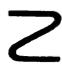
\includegraphics[keepaspectratio]{images/part001_c7194320.jpg}}

我们注意到，若 M 与 N 是 Hausdorff 拓扑向量空间 E 中任意两个闭向量子空间，则 \(M + N\) 在 E 中不一定是闭的，* 即使 E 是 Hilbert 空间 *（cf.~IV, 第 64 页, 习题 13, d)）。

命题 3. --- 设 E 是完备非离散赋值除环 K 上的一个拓扑向量空间。设 M 是 E 中具有有限余维数 n 的闭向量子空间。则 M 在 E 中的每个代数补子空间 N 也是拓扑补。

在 N 中，集合 \(\{0\}\) 是闭的，因为它是 N 与在 E 中为闭的集合 M 的交；于是 N 是 Hausdorff 的。由于 E/M 也是 Hausdorff 的，N 到 E/M 上的典范映射（它线性且双射）是双连续的（I, 第 14 页, cor. 2），由此命题得证。

推论. --- 设 E 与 F 是完备非离散赋值除环上的两个拓扑向量空间。若 F 是 Hausdorff 的且有限维，则 E 到 F 上的每个连续线性映射都是严格态射。

注记. --- 第 2, 3 目的结果当 K 是离散除环时不再成立。例如，设 \(K_{1}\) 是非离散赋值除环，K 是通过给 \(K_{1}\) 赋以 \(K_{1}\) 上的非真绝对值而得到的离散除环。于是 \(K_{1}\) 是 K 上的一个一维拓扑向量空间，但它不同构于 \(K_{s}\)。不过，我们可以证明：只要对所考虑的拓扑向量空间加上具有 0 的均衡邻域基本系这一性质（即满足 \(K.V = V\) 的邻域 V）（I, 第 27 页, 习题 14），第 2, 3 目的结果即使当 K 是离散的也成立；正如上例所示，这一条件（当 K 是非离散赋值除环时它总被满足，cf.~I, 第 7 页, prop. 4）并非对 K 上的所有拓扑向量空间都成立。

\subsection{局部紧拓扑向量空间}

定理 3. --- 设 K 是完备非离散赋值除环。若 E 是 K 上的一个 Hausdorff 拓扑向量空间，且 E 中 0 的某个邻域 V 是预紧的，则 E 是有限维的。若 \(E \neq \{0\}\)，则 K 与 E 都是局部紧的。

在证明第一个论断时，只需考虑 E 是完备的情形；因为 E 是其完备化 \(\hat{E}\) 的一个处处稠密的子空间，且 V 的闭包 \(\overline{V}\)（取在 \(\hat{E}\) 中）是紧的，并且是 \(\hat{E}\) 中 0 的一个邻域（GT, III, § 3.4, prop. 7）。

于是可以假设 E 中 0 有一个紧邻域 V。设 \(\alpha \in \mathbf{K}\) 满足 \(0 < |\alpha| < 1\)；则存在有限多个点 \(a_i \in \mathbf{V}\) 使得

\[
\mathrm{V} \subset \bigcup_ {i} (a _ {i} + \alpha \mathrm{V}).
\]

设 M 是 E 中由诸 \(a_{i}\) 生成的有限维子空间；它在 E 中是闭的（I, 第 14 页, cor. 1）。在 Hausdorff 拓扑向量空间 E/M 中，V 的典范像 W 是 0 的一个紧邻域，满足 \(W \subset \alpha W\)；由此 \(\alpha^{-1} W \subset W\)，并且对 n 作归纳可得：对每个正整数 n 有 \(\alpha^{-n} W \subset W\)。由于 W 是吸收的，我们断言 W = E/M；从而 E/M 是紧的。因此，要完成定理中第一个论断的证明，只需证明下述引理。

引理 1. --- 非离散赋值除环上的每个紧拓扑向量空间 E 都恰好是集合 \(\{0\}\)。

由于 E 是完备的，可以假设 K 是完备的（I, 第 6 页）。若 \(E \neq \{0\}\)，则 E 含有一条在 E 中闭的直线（I, 第 14 页, cor. 1），从而这条直线是紧的。这条直线同构于 \(K_{s}\)（I, 第 12 页, prop. 2），因而 K 必是紧的。但映射 \(\xi \mapsto |\xi|\)（K 到 R 中的映射）是连续的，故 K 的像必有界；另一方面，存在 \(\gamma \in K\) 使 \(|\gamma| > 1\)，而集合 \(|\gamma^{n}| = |\gamma|^{n}\)（\(n \in N\)）是无界的。这一矛盾表明 \(E = \{0\}\)。

为证明定理中的第二个论断，若 \(E \neq \{0\}\)，则由定理的第一部分，E 同构于 \(K_{s}^{n}\)，其中 n \textgreater{} 0；而 K 是完备的，故 E 也是完备的，从而 E 是局部紧的。但 \(K_{s}\) 同构于 E 中的一条直线（I, 第 12 页, prop. 2），后者在 E 中必然是闭的（I, 第 14 页, cor. 1）；由此推出 K 是局部紧的。

注记. --- 当 K 是离散除环时，th. 3 的结果不再成立，正如把 R（取通常拓扑）视为离散域 Q 上的拓扑向量空间这一例子所示。

\section{可度量化拓扑向量空间}

\subsection{可度量化拓扑向量空间中 0 的邻域}

我们称拓扑向量空间 E 是可度量化的，如果它的拓扑是可度量化的。相对于其加群的结构与其拓扑，E 因此是一个可度量化群（GT, IX, § 3.1）。

我们知道，为使一个拓扑群可度量化，必须且只需存在中性元 e 的一个可数的基本邻域系，它的交是单个元素 e（GT, IX, § 3.1, prop. 1）。

我们也知道，可度量化拓扑向量空间 E 的一致结构可以由一个不变距离 \(d(x, y) = |x - y|\) 定义，其中 \(x \mapsto |x|\) 是 E 到 \(R_{+}\) 中的一个连续映射，且满足条件：1) \(|-x| = |x|\)；2) \(|x + y| \leqslant |x| + |y|\)；3) 关系 \(|x| = 0\) 等价于 x = 0（GT, IX, § 3.1, prop. 3）。

我们已经看到（GT, IX, § 3.1, prop. 2），如何定义这样一个距离 \(d\)（利用 E 中 0 的邻域的一个递减序列 \((\mathbf{W}_n)\)），该序列构成一个基本邻域系，且满足 \(\mathbf{W}_{n+1} + \mathbf{W}_{n+1} + \mathbf{W}_{n+1} \subset \mathbf{W}_n\)。当 E 是非离散赋值除环 K 上的可度量化向量空间时，还可以假设诸 \(\mathbf{W}_n\) 是均衡的（I, 第 7 页, prop. 4）；回到 \(d\) 的定义过程（loc. cit.），我们可以看出关系 \(|\lambda| \leqslant 1\) 蕴含 \(|\lambda x| \leqslant |x|\)。此外，I, 第 2 页 的条件 (EVT \(_i\)) 与 (EVT \(_ii\)) 既蕴含 \(|\lambda x_0|\)（当 \(\lambda\) 在 K 中趋于 0 时，对每个 \(x_0 \in \mathrm{E}\)）趋于 0，又蕴含 \(|\lambda_0 x|\)（当 \(|x|\) 趋于 0 时，对每个 \(\lambda_0 \in \mathrm{K}\)）趋于 0。反之，若函数 \(|x|\) 具有前述所有性质，且 \(\mathbf{W}_n\) 是由 \(x \in \mathrm{E}\)（满足 \(|x| \leqslant 2^{-n}\)）所成的集合，则诸 \(\mathbf{W}_n\) 构成 E 上与 E 的向量空间结构相容的某个可度量化拓扑的 0 的均衡邻域基本系。

注记. --- 最重要的可度量化向量空间类之一是赋范空间（I, 第 3 页）。但必须注意，存在其拓扑不能用范数定义的可度量化向量空间（I, § 3, 习题 1）；我们稍后将研究一些重要的例子。

\subsection{可度量化向量空间的性质}

可度量化拓扑向量空间 E 的每个向量子空间都是可度量化的；E 关于闭向量子空间 M 的每个商空间 E/M 亦然（GT, IX, § 3.1, prop. 4）。可度量化拓扑向量空间的可数族的每个乘积都是可度量化的（GT, IX, § 2.4, cor. 2）。若 \(K_{0}\) 是完备赋值除环，K 是在 \(K_{0}\) 中处处稠密的一个子除环，则 K 上的可度量化向量空间 E 的完备化 \(\hat{E}\) 是 \(K_{0}\) 上的一个可度量化向量空间（I, 第 6 页 及 GT, IX, § 2, No.~1, prop. 1）。最后，若 E 是完备的可度量化向量空间，则对 E 的每个闭向量子空间 M，商空间 E/M 是完备的（GT, IX, § 3.1, prop. 4）。

\subsection{可度量化向量空间中的连续线性函数}

定理 1 (Banach). --- 设 E 与 F 是非离散赋值除环 K 上的两个可度量化向量空间，并设 u 是 E 到 F 中的一个连续线性映射。假设 E 是完备的。则下列条件等价：

\begin{enumerate}
\def\labelenumi{(\roman{enumi})}
\item
  \(u\) 是一个严格满射态射。
\item
  F 是完备的且 \(u\) 是满射。
\item
  \(u\) 的像在 \(\mathbf{F}\) 中不是贫集（GT, IX, § 5.2）。
\item
  对 0 的每个邻域 \(\mathbf{V}\)（在 \(\mathbf{E}\) 中），集合 \(\overline{u(\mathbf{V})}\) 是 0 在 \(\mathbf{F}\) 中的一个邻域。首先 (i) 蕴含 (ii)，因为设 \(u\) 是一个严格满射态射，\(\mathbf{N}\) 是 \(u\) 的核。则 \(u\) 诱导 \(\mathrm{E/N}\) 到 \(\mathbf{F}\) 上的一个同构。但 \(\mathbf{E}\) 是可度量化且完备的，故 \(\mathrm{E/N}\) 是完备的（GT, IX, § 3.1, prop. 4），因此 \(\mathbf{F}\) 是完备的。
\end{enumerate}

其次 (ii) 蕴含 (iii)。设 F 是完备的且 u 是满射。u 的像恰好是 F，因而由 Baire 定理（GT, IX, § 5.3）它在 F 中不是贫集。

下述引理表明 (iii) 蕴含 (iv)。

引理 1. --- 设 E 与 F 是非离散赋值除环 K 上的两个拓扑向量空间，并设 u 是 E 到 F 中的一个连续线性映射，且 E 的像不是贫集。则对 E 中 0 的每个邻域 V，集合 \(\overline{u(V)}\) 是 F 中 0 的一个邻域。

设 W 是 E 中 0 的一个均衡邻域，满足 \(W + W \subset V\)（I, § 1.5, prop. 4）。设 \(\alpha\) 是 K 中满足 \(|\alpha| > 1\) 的一个元素；则 E 是诸集合 \(\alpha^{n}W\)（其中 n 取遍 N）的并；事实上，对每个 \(x \in E\)，存在 \(\beta \in K\) 使 \(x \in \beta W\)（I, 第 7 页, prop. 4），且存在整数 \(n \geqslant 0\) 使 \(|\beta| < |\alpha|^{n}\)，于是由 W 是均衡的，得 \(x \in \alpha^{n}W\)。因此，\(u(E)\) 是集合序列 \(u(\alpha^{n}W) = \alpha^{n}u(W)\) 的并；由于 \(u(E)\) 在 F 中不是贫集，诸集合 \(\alpha^{n}\overline{u(W)}\) 中至少有一个具有内点（GT, IX, § 5.3, def. 2），从而 \(\overline{u(W)}\) 具有内点。

设 \(y_0\) 是 \(\overline{u(\mathbf{W})}\) 的一个内点；由于 \(-u(\mathbf{W}) = u(\mathbf{W})\)，从而 \(-\overline{u(\mathbf{W})} = \overline{u(\mathbf{W})}\)，由此得出 \(0 = y_0 + (-y_0)\) 是 \(\overline{u(\mathbf{W})} + \overline{u(\mathbf{W})}\) 的一个内点。由于向量加法是 \(F \times F\) 到 \(F\) 中的连续映射，集合 \(\overline{u(\mathbf{W})} + \overline{u(\mathbf{W})}\) 包含在集合

\[
u (\mathrm{W}) + u (\mathrm{W}) = u (\mathrm{W} + \mathrm{W}) \subset u (\mathrm{V});
\]

的闭包之中；因此 \(\overline{u(\mathrm{V})}\) 是 F 中 0 的一个邻域。

在证明 (iv) 蕴含 (i) 之前，我们先证明下述引理，其中我们约定：在所有度量空间中，\(\mathbf{B}_{r}(x)\) 表示以 x 为中心、以 r 为半径的闭球。

引理 2. --- 设 E 与 F 是两个度量空间，且假设 E 还是完备的。设 u 是 E 到 F 中的一个线性映射，具有下述性质：无论数 r \textgreater{} 0 如何，都存在一个数 \(\rho(r) > 0\)，使得对每个 \(x \in E\)，我们有

\[
\mathrm{B} _ {\rho (r)} (u (x)) \subset \overline {{u (\mathrm{B} _ {r} (x))}}.
\]

在这些条件下，对每个 \(a > r\)，像 \(u(\mathbf{B}_a(x))\) 包含球 \(\mathbf{B}_{\rho(r)}(u(x))\)。

设 \((r_n)\) 是一个无穷的数列 \(>0\)，满足 \(r_1 = r\) 且 \(a = \sum_{n=1}^{\infty} r_n\)。对每个指标 \(n\)，存在一个数 \(\rho_n > 0\)（其中 \(\rho_1 = \rho(r)\)）使得

\[
\mathrm{B} _ {\rho_ {n}} (u (x)) \subset \overline {{u (\mathrm{B} _ {r _ {n}} (x))}}
\]

对每个 \(x \in E\)；我们可以而且将假设 \(\lim \rho_{n} = 0\)。

设 \(x_0\) 是 \(E\) 的一个点，\(y\) 是 \(B_{\rho(r)}(u(x_0))\) 的一个点。我们将证明 \(y\) 属于 \(u(B_a(x_0))\)。

为此，对 E 的点归纳地定义一个序列 \((x_{n})_{n>0}\)，使得对每个 \(n \geqslant 1\)，有 \(x_{n} \in \mathbf{B}_{r_{n}}(x_{n-1})\) 且 \(u(x_{n}) \in \mathbf{B}_{\rho_{n+1}}(y)\)。若诸 \(x_{i}\) 已对 \(0 \leqslant i \leqslant n - 1\) 按满足这些关系的方式定义好，则我们有 \(y \in \mathbf{B}_{\rho_{n}}(u(x_{n-1}))\)；由于

\[
\mathrm{B} _ {\rho_ {n}} (u (x _ {n - 1})) \subset \overline {{u (\mathrm{B} _ {r _ {n}} (x _ {n - 1}))}},
\]

则存在一个点 \(x_{n} \in \mathbf{B}_{r_n}(x_{n-1})\)，它的像 \(u(x_{n})\) 属于邻域 \(\mathbf{B}_{\rho_{n+1}}(y)\)（\(y\) 的邻域），这就确立了序列 \((x_{n})\) 的存在性。

由于 \(x_{n}\) 与 \(x_{n+p}\) 的距离小于 \(r_{n+1} + r_{n+2} + \cdots + r_{n+p}\)（当 n 充分大时它可任意小），序列 \((x_{n})\) 是 E 中的 Cauchy 序列。由于 E 是完备的，序列 \((x_{n})\) 收敛于 E 的一个点 x。\(x_{0}\) 与 x 的距离小于 \(\sum_{n=1}^{\infty} r_{n} = a\)，从而 \(x \in \mathbf{B}_{a}(x_{0})\)。但 u 是连续的，故序列 \(u(x_{n})\) 收敛于 \(u(x)\)；又有 \(u(x_{n}) \in \mathbf{B}_{\rho_{n+1}}(y)\)，因此 \(y = u(x)\)，引理得证。

我们回到定理并证明 (iv) 蕴含 (i)。设 \(u\) 满足条件 (iv)。对空间 E 与 F 中的每一个，取一个在平移下不变且定义其拓扑的距离（I, 第 16 页）。根据假设，集合 \(u(\mathbf{B}_r(0))\) 对每个 \(r > 0\) 都是 F 中 0 的邻域，从而存在一个数 \(\rho(r) > 0\) 使 \(\mathbf{B}_{\rho(r)}(0) \subset u(\mathbf{B}_r(0))\)。通过平移我们断言：\(\mathbf{B}_{\rho(r)}(u(x)) \subset u(\mathbf{B}_r(x))\) 对每个 \(r > 0\) 及每个 \(x \in E\) 成立。由引理 2，对每一对正实数 \((a, r)\)（\(a > r > 0\)），我们有 \(\mathbf{B}_{\rho(r)}(0) \subset u(\mathbf{B}_a(0))\)；因此 \(u\) 是 E 到 F 上的一个严格态射。我们已证明 (iv) 蕴含 (i)，定理的证明至此完成。

推论 1. --- 若 E 与 F 是非离散赋值除环上的两个完备可度量化向量空间，则 E 到 F 上的每个双射连续线性映射都是同构。

特别地，若 E 与 F 是两个完备赋范空间，则存在一个数 \(a > 0\)，使得 \(\| u(x)\| \geqslant a.\| x\|\) 对每个 \(x\in \mathbf{E}\) 成立。

推论 2. --- 设 E 是非离散赋值除环上的一个向量空间，\(T_{1}\) 与 \(T_{2}\) 是 E 上与其向量空间结构相容的两个拓扑，且对其中每个拓扑 E 都是可度量化且完备的。则若 \(T_{1}\) 与 \(T_{2}\) 可比较，它们就恒同。

推论 3. --- 设 E 与 F 是非离散赋值除环上的两个完备可度量化向量空间。为使 E 到 F 中的一个连续线性映射 u 是严格态射，必须且只需 \(u(\mathrm{E})\) 在 F 中是闭的。

该条件是必要的，因为若 u 是严格态射，则像 \(u(\mathrm{E})\) 同构于商 \(\mathrm{E}/u^{-1}(0)\)，因而是完备的（I, 第 17 页），从而在 F 中是闭的。该条件是充分的，因为若 \(u(\mathrm{E})\) 在 F 中是闭的，则 \(u(\mathrm{E})\) 必是一个完备可度量化向量空间，从而由定理 1，u 是 E 到 \(u(\mathrm{E})\) 上的一个严格态射。

推论 4. --- 设 E 是非离散赋值除环上的一个完备可度量化向量空间。若 M 与 N 是 E 的两个闭向量子空间，且它们在 E 中（代数）互补，则 E 是 M 与 N 的拓扑直和。

因为 \(M \times N\) 是完备可度量化向量空间，且映射 \((y, z) \mapsto y + z\)（\(M \times N\) 到 E 上的映射）连续且双射，从而是同构（cor. 1）。

推论 5 (闭图像定理). --- 设 E 与 F 是非离散赋值除环上的两个完备可度量化向量空间。为使 E 到 F 中的一个线性映射 u 连续，必须且只需它的图在乘积空间 \(E \times F\) 中是闭的。

该条件是必要的，因为到 Hausdorff 空间中的连续映射的图是闭的（GT, I, § 8.1, cor. 2）。为看出它是充分的，注意它蕴含：u 的图 G（它是完备可度量化空间 \(E \times F\) 的一个闭向量子空间）本身是可度量化的且完备的。G 到 E 上的投影 \(z \mapsto \operatorname{pr}_{1}(z)\) 是一个双射的连续线性映射，从而是同构（cor. 1）；由于它的逆映射是 \(x \mapsto (x, u(x))\)，由此得出 \(u\) 在 E 中连续。

我们可以把这个推论表述成如下形式：\(u\) 是连续的，如果下述情形成立：若 E 的点的序列 \((x_{n})\) 既收敛于 0，又使序列 \((u(x_{n}))\) 收敛于 \(y\)，则必然有 \(y = 0\)。

例. --- 设 E 是定义在 I = \([0, 1]\) 上的实值函数所成空间的一个向量子空间；设 \(\|f\|\) 是 E 上的一个范数，在此范数下 E 是完备的，且使得 E 的拓扑比简单收敛拓扑更细。进一步假设 E 包含在 I 上无穷次可微的函数所成的集合 \(\mathcal{C}^{\infty}(\mathrm{I})\)；我们将证明存在一个整数 \(k \geqslant 0\)，使 E 包含在 I 中具有连续的 k 阶导数的所有函数所成的集合 \(\mathcal{C}^{k}(\mathrm{I})\)。

对每一对整数 \(m > 0\), \(n \geqslant 0\)，设 \(V_{mn}\) 是由那些 \(f \in \mathcal{C}^{\infty}(\mathrm{I})\)（满足 \(|f^{(h)}(x)| \leqslant 1 / m\)，其中 \(0 \leqslant h \leqslant n\) 且对每个 \(x \in \mathrm{I}\)）所成的集合。诸 \(V_{m,n}\) 构成与 \(\mathcal{C}^{\infty}(\mathrm{I})\) 的向量空间结构相容的某个可度量化拓扑的 0 的一个基本邻域系，此外 \(\mathcal{C}^{\infty}(\mathrm{I})\) 在此拓扑下是完备的（FVR, II, 第 2 页, th. 1）。设 \(u\) 是 \(\mathcal{C}^{\infty}(\mathrm{I})\) 到 E 中的典范映射；我们证明 \(u\) 连续。由上面的 cor. 5，只需证明：若一个序列 \((f_n)\) 在 \(\mathcal{C}^{\infty}(\mathrm{I})\) 中收敛于 0 且在 E 中收敛于一个极限 \(f\)，则必然 \(f = 0\)。但这是直接的，因为根据假设，\(f\) 是 \((f_n)\) 的简单收敛极限。因此存在一个整数 \(k \geqslant 0\) 和一个数 \(a > 0\)，使得关系

\[
p_{k}(f) = \sup_{\substack{x\in \mathbf{I}\\ 0\leqslant h\leqslant k}}\big|f^{(h)}(x)\big|\leqslant a
\]

蕴含 \(\| f\| \leqslant 1\)，对每个 \(f\in \mathcal{C}^{\infty}(\mathrm{I})\)

但 \(p_k\) 是空间 \(\mathcal{C}^k(\mathrm{I})\) 上的一个范数，且对此范数 \(\mathcal{C}^\infty(\mathrm{I})\) 是在 \(\mathcal{C}^k(\mathrm{I})\) 中处处稠密的一个子空间（多项式的集合已在 \(\mathcal{C}^k(\mathrm{I})\) 中处处稠密，这是 Weierstrass-Stone 定理的一个直接推论）。由前所述，\(\mathcal{C}^\infty(\mathrm{I})\)（带范数 \(p_k\)）到 \(\mathrm{E}\) 中的恒等映射是连续的，因而它可以连续地延拓到整个空间 \(\mathcal{C}^k(\mathrm{I})\)（因为 \(\mathrm{E}\) 是完备的）。这就证明了我们的断言。

命题 1. --- 设 E, F 是非离散赋值除环 K 上的两个拓扑向量空间。我们假设：

\begin{enumerate}
\def\labelenumi{\arabic{enumi})}
\item
  E 是可度量化且完备的。
\item
  存在 K 上的完备可度量化向量空间的一个序列 \((\mathbf{F}_{n})\)，且对每个 n，存在一个单射连续线性映射 \(v_{n}\)（\(F_{n}\) 到 F 中的映射），使得 F 是诸子空间 \(v_{n}(\mathbf{F}_{n})\) 的并。
\end{enumerate}

再设 u 是 E 到 F 中的一个线性映射。若 u 的图在 \(E \times F\) 中是闭的，则存在一个整数 n 和一个连续线性映射 \(u_{n}\)（E 到 \(F_{n}\) 中的映射），使得 \(u = v_{n} \circ u_{n}\)（这蕴含 u 连续且 \(u(\mathrm{E}) \subset v_{n}(\mathrm{F}_{n})\)）。

设 G 是 u 在 \(E \times F\) 中的图。对每个 n，我们考虑连续线性映射 \(w_{n}:(x,y)\mapsto(x,v_{n}(y))\)（\(E \times F_{n}\) 到 \(E \times F\) 中的映射）；由于 G 是闭的，集合 \(w_{n}^{-1}(\mathbf{G})=\mathbf{G}_{n}\) 是 \(E \times F_{n}\) 的一个闭向量子空间；若 \(p_{n}\) 是 \(G_{n}\) 上的限制映射，即第一投影 \(pr_{1}\) 的限制，则我们有 \(p_{n}(\mathbf{G}_{n})=u^{-1}(v_{n}(\mathbf{F}_{n}))\)。由于 \(p_{n}\) 连续且 \(G_{n}\) 完备（因为 \(G_{n}\) 在完备空间 \(E \times F_{n}\) 中是闭的），由定理 1，\(p_{n}(\mathbf{G}_{n})\) 或者在 E 中是贫集，或者是整个 E。但根据假设，E 是诸 \(p_{n}(\mathbf{G}_{n})\) 的并，且由于 E 是完备的，由 Baire 定理（GT, IX, § 5.3, th. 1），诸 \(p_{n}(\mathbf{G}_{n})\) 不可能全是 E 中的贫集。因此存在一个整数 n 使 \(p_{n}(\mathbf{G}_{n}) = \mathbf{E}\)，换言之 \(u(\mathbf{E}) \subset v_{n}(\mathbf{F}_{n})\)。此外，由于 \(v_{n}\) 是单射，\(G_{n}\) 是某个线性映射 \(u_{n}\)（E 到 \(F_{n}\) 中的映射）的图，且由闭图像定理（I, 第 19 页, cor. 5）\(u_{n}\) 连续；于是由定义可得 \(u = v_{n} \circ u_{n}\)。

\exercisesheading

\exercisegroup

\begin{enumerate}
\def\labelenumi{\arabic{enumi})}
\item
  设 \(E_{0}=Q_{p}^{N}\) 是 p 进域 \(Q_{p}\)（GT, III, § 6, 习题 23）上的向量空间，它是由每个都恒等于 \(Q_{p}\) 的因子所组成的可数无穷乘积。设 \(P\subset E_{0}\) 是集合 \(Z_{p}^{N}\)，并设 E 是由 P 生成的 \(E_{0}\) 的向量子空间。在加群 P 上我们考虑诸因子 \(Z_{p}\) 的拓扑的乘积紧拓扑，并用 B 表示 P 关于此拓扑的 0 的邻域滤子。证明：B 是 E 上某个与 E 的加群结构相容的拓扑 T 的 0 的基本邻域系，该拓扑满足 \((\mathrm{EVT}_{\mathrm{I}}^{\prime})\) 与 \((\mathrm{EVT}_{\mathrm{III}}^{\prime})\) 但不满足 \((\mathrm{EVT}_{\mathrm{II}}^{\prime})\)（证明位似 \(x\mapsto x/p\) 在 E 中不连续）。
\item
  设 K 是非离散拓扑除环，\(K_{0}\) 是赋以离散拓扑的除环 K。\(K_{0}\) 上的离散拓扑与其加群结构相容，且当我们把 \(K_{0}\) 看作 K 上的向量空间时，它满足公理 (EVT \(_{II}\)) 与 (EVT \(_{III}\)) 但不满足 (EVT \(_{I}\))。
\item
  对每个实数 \(\alpha > 0\)，设 \(G_{\alpha}\) 是拓扑群 \(\mathbf{R} / \alpha \mathbf{Z}\)，并设 \(G\) 是拓扑乘积群 \(\prod_{\alpha} G_{\alpha}\)（\(\alpha\) 取遍数 \(>0\) 组成的集合）。对每个 \(x \in \mathbf{R}\)，
\end{enumerate}

设 \(t_{\alpha}(x)\) 是 \(x\) 在 \(G_{\alpha}\) 中的典范像；映射 \(\phi : x \to (t_{\alpha}(x))\) 是 \(\mathbf{R}\) 到 \(G\) 中的一个连续单射同态。我们在 \(\mathbf{R}\) 上考虑由 \(\phi\) 取的 \(G\) 的拓扑的原像拓扑，并用 \(E\) 表示由赋以此拓扑的 \(\mathbf{R}\) 所成的拓扑群。证明：当把 \(E\) 看作 \(\mathbf{R}\) 上的向量空间时，其拓扑满足 \((\mathrm{EVT}_{I}^{\prime})\) 与 \((\mathrm{EVT}_{II}^{\prime})\) 但不满足 \((\mathrm{EVT}_{III}^{\prime})\)。

\begin{enumerate}
\def\labelenumi{\arabic{enumi})}
\setcounter{enumi}{3}
\item
  设 E 是带赋值的除环 K 上的一个向量空间；假设 E 带有与其加群结构相容的一个可度量化拓扑。进一步假设此拓扑满足公理 (EVT \(_{I}\)) 与 (EVT \(_{II}\))；证明：若两个可度量化群 K, E 中有一个是完备的，则该拓扑也满足 (EVT \(_{III}\))，从而与 E 的向量空间结构相容（cf.~GT, IX, § 5, 习题 23）。
\item
  设 \(\mathbf{K}\) 是非离散赋值域，\(S\) 是任意一个无穷集合。
\end{enumerate}

\begin{enumerate}
\def\labelenumi{\alph{enumi})}
\item
  设 \(\mathbf{D} = (a_n)\) 是 \(\mathbf{S}\) 的元素的一个可数无穷族。对每个 \(\lambda \in \mathbf{K}\)（满足 \(|\lambda| \leqslant 1\)），设 \(u_{\lambda}\) 是赋范空间 \(\mathcal{B}_{\mathbf{K}}(\mathbf{S})\)（I, 第 4 页, 例；该空间由 \(\mathbf{S}\) 到 \(\mathbf{K}\) 中的有界映射组成）的元素，满足 \(u_{\lambda}(a_n) = \lambda^n\)（对每个 \(n \in \mathbf{N}\)），且 \(u_{\lambda}(b) = 0\)（对每个 \(b \notin \mathbf{D}\)）。证明族 \((u_{\lambda})\) 是代数无关的。
\item
  推出向量空间 \(\mathcal{B}_{\mathbf{K}}(\mathbf{S})\) 的每个基与 \(\mathrm{K}^{\mathrm{s}}\) 有相同的基数（利用 \(a\)），证明 \(\mathcal{B}_{\mathbf{K}}(\mathbf{S})\) 的每个基的基数至少等于 Card (K)；另一方面注意 \(\operatorname{Card}(\mathcal{B}_{\mathbf{K}}(\mathbf{S})) = \operatorname{Card}(\mathbf{K}^{\mathrm{s}})\) 并利用 A, II, § 2, 习题 22）。
\item
  以同样的方式证明向量空间 \(\ell_{\mathbf{K}}^{1}(\mathbf{S})\) 的每个基具有 \((\mathbf{K}\times \mathbf{S})^{\mathbf{N}}\) 的基数。
\end{enumerate}

\begin{enumerate}
\def\labelenumi{\arabic{enumi})}
\setcounter{enumi}{5}
\tightlist
\item
  设 \(\mathbf{K}\) 是非离散赋值除环。证明：对空间 \(\ell_{\mathbf{K}}^{1}(\mathbf{N})\)（由形如 \(x = (\xi_n)\) 的、由 \(\mathbf{K}\) 中元素组成的绝对可和序列构成）而言，范数 \(\| x \|_1 = \sum_{n=0}^{\infty} |\xi_n|\) 与 \(\| x \| = \sup_n |\xi_n|\) 不等价（cf.~GT, IX, § 3.3, prop. 7）；证明 \(\ell_{\mathbf{K}}^{1}(\mathbf{N})\)（带范数 \(\| x \|\)）从不完备，即使 \(\mathbf{K}\) 是完备的；它在 \(\mathcal{B}_{\mathbf{K}}(\mathbf{N})\) 中的闭包是什么？
\end{enumerate}

¶ 7) * 设 A 是一个离散赋值环，v 是 A 的分式除环 K 的赋范赋值；在 K 上取绝对值 \(a^{v}\)，其中 0 \textless{} a \textless{} 1。设 E 是 K 上的一个赋范向量空间，其范数满足超度量不等式

\[
\| x + y \| \leqslant \sup (\| x \|, \| y \|).
\]

\begin{enumerate}
\def\labelenumi{\alph{enumi})}
\item
  用 M 表示由那些 \(x \in E\)（满足 \(\| x \| \leqslant 1\)）所组成的集合，用 \(\pi\) 表示 A 的一个单值化元；M 是一个 A-模，而 \(M / \pi M\) 是 A 的剩余除环 \(k = A / \pi A\) 上的一个向量空间。设 \((e_{\lambda})_{\lambda \in L}\) 是 M 的元素的一个族，使得诸 \(e_{\lambda}\) 在 \(M / \pi M\) 中的像构成这个 \(k\) -向量空间的一个基。证明 \((e_{\lambda})\) 是 E 中的一个无关族，且由 \((e_{\lambda})\) 生成的 E 的向量子空间 F 在 E 中稠密。
\item
  若置 \(\| x\| _1 = \sup_{\lambda}|\xi_\lambda |,\)（对 F 中每个 \(x = \sum_{\lambda}\xi_{\lambda}e_{\lambda}\)），证明在 F 上范数 \(\| x\|\) 与 \(\| x\| _1\) 等价。
\item
  设 \(\mathbf{K}\) 是完备的。由 \(a)\) 与 \(b)\) 推出：若 \(\mathbf{L}\) 有限，则完备化 \(\hat{\mathbf{E}}\)（即 \(\mathbf{E}\) 的完备化）同构于 \(\mathbf{K}^{\mathrm{L}}\)；若 \(\mathbf{L}\) 无限，则 \(\hat{\mathbf{E}}\) 同构于子空间 \(\mathcal{C}_{\mathbf{K}}^{0}(\mathbf{L})\)，即 \(\mathcal{B}_{\mathbf{K}}(\mathbf{L})\) 中由那些族 \((\xi_{\lambda})\)（它们满足 \(\lim \xi_{\lambda} = 0\)，关于 \(\mathbf{L}\) 的有限子集的补集所组成的滤子）所组成的子空间。
\item
  假设 K 与 E 完备；设 G 是 K 上另一个完备赋范空间，其范数满足超度量不等式。证明：在（如有必要）把 \(\mathcal{L}(\mathrm{E};\mathrm{G})\)（GT, X, § 3.2）的范数换成一个等价的范数之后，\(\mathcal{L}(\mathrm{E};\mathrm{G})\) 等距同构于由 G 中元素组成的诸族 \((y_{\lambda})_{\lambda \in L}\)（它们满足 \(\sup_{\lambda \in L}\| y_{\lambda}\| < +\infty\)）所成的向量空间，后者带范数 \(\sup_{\lambda \in L}\| y_{\lambda}\|\)（它也是一个超度量范数）。
\end{enumerate}

\begin{enumerate}
\def\labelenumi{\arabic{enumi})}
\setcounter{enumi}{7}
\item
  设 E 是非离散拓扑除环 K 上的一个拓扑向量空间。为使存在点 \((0,0)\)（在 \(K \times E\) 中）的一个邻域，使映射 \((\lambda, x) \mapsto \lambda x\) 在此邻域上一致连续，必须且只需存在 E 中 0 的一个邻域 \(V_{0}\)，使得诸集合 \(\lambda V_{0}\)（其中 \(\lambda\) 取遍 K 中 \(\neq 0\) 的元素）构成 E 中 0 的一个基本邻域系。当 K 是非离散赋值除环且 E 是 Hausdorff 的时，证明 E 的一致结构此时是可度量化的。
\item
  把 I, 第 8 页 的 prop. 5 推广到如下的情形：诸空间 \(\mathrm{E}_i\)（\(\leqslant i \leqslant n\)）与 \(\mathrm{F}\) 是任意非离散拓扑域上的拓扑向量空间。
\item
  设 E 是非离散赋值除环 K 上的一个完备 Hausdorff 拓扑向量空间。用 F 表示 E 的一个向量子空间，用 T 表示 F 上由 E 的拓扑 \(T'\) 诱导的拓扑；设 B 是拓扑 T 的 0 的闭均衡邻域的一个基本系。设 \(F_{0}\) 是 E 的向量子空间，由闭包 \(\overline{V}\)（在 E 中关于 \(T'\) 取的、诸集合 \(V \in B\) 的闭包）生成；诸集合 \(\overline{V}\) 构成某个拓扑 \(T_{0}\)（\(F_{0}\) 上的拓扑）的 0 的一个基本邻域系，该拓扑与 \(F_{0}\) 的向量空间结构相容；对此拓扑，\(F_{0}\) 是完备的，且 \(T_{0}\) 在 F 上诱导的拓扑与 T 恒同。
\item
  在非离散拓扑除环 K 上的拓扑向量空间 E 中，存在 0 的闭邻域的一个基本系 B，满足条件 (EV \(_{II}\)) 与 (EV \(_{III}\)) 以及下面两个：
\end{enumerate}

\((\mathrm{EV}_{\mathrm{Ia}})\) 对每个 \(\mathbf{V} \in \mathfrak{B}\)，存在 \(\mathbf{W} \in \mathfrak{B}\) 以及 0 的一个邻域 \(\mathbf{U}\)（\(\mathbf{K}\) 中的邻域），使得 \(\mathrm{UW} \subset \mathrm{V}\)。\((\mathrm{EV}_{\mathrm{Ib}})\) 对每个 \(x \in \mathbf{E}\) 及每个 \(\mathbf{V} \in \mathfrak{B}\)，存在 \(\lambda \neq 0\)（\(\mathbf{K}\) 中的元素），使得 \(\lambda x \in \mathbf{V}\)。反之，设 \(\mathbf{E}\) 是 \(\mathbf{K}\) 上的一个向量空间，并设 \(\mathfrak{B}\) 是 \(\mathbf{E}\) 上满足条件 \((\mathrm{EV}_{\mathrm{Ia}}), (\mathrm{EV}_{\mathrm{Ib}}), (\mathrm{EV}_{\mathrm{II}})\) 与 \((\mathrm{EV}_{\mathrm{III}})\) 的一个滤子基。证明 \(\mathbf{E}\) 上存在（且仅存在一个）与 \(\mathbf{E}\) 的向量空间结构相容的拓扑，使 \(\mathfrak{B}\) 是它的 0 的基本邻域系。

\begin{enumerate}
\def\labelenumi{\arabic{enumi})}
\setcounter{enumi}{11}
\item
  设 K 是离散域，E 是 K 上两个未定元的形式级数环 A = K{[}{[}X, Y{]}{]}（A, IV, 第 36 页）的分式除环。对每个 \(n \geqslant 0\)，设 \(V_{n} \subset A\) 是总次数至少等于 n 的形式级数所成的集合。证明：在 E 中，诸集合 \(V_{n}\) 构成 0 的一个基本邻域系，对应于与 E（在 K 上）的向量空间结构相容的一个拓扑，对此拓扑 E 是可度量化且完备的；若进一步 K 是有限域，则 E 是局部紧的。证明 E × E 到 E 中的 K-双线性映射 \((u, v) \mapsto uv\) 在点 \((0, 0)\) 处连续，但存在 \(u_{0} \in E\) 使 \(v \mapsto u_{0}v\) 在 E 中不连续（例如 \(u_{0} = 1/X\)）。
\item
  设 E 是 R 上无穷维的一个向量空间，并设 T 是 E 的所有吸收集与均衡集所成的族。证明 T 不满足公理 \((\mathrm{EV}_{\mathrm{III}})\)（换言之，不是与 E 的加群结构相容的某个拓扑的 0 的基本邻域系）。为此，考虑 E 中一个无穷无关族 \((e_{n})_{n\geqslant1}\)；对每个整数 \(n\geqslant1\)，设 \(A_{n}\) 是形如 \(\sum_{i=1}^{n}t_{i}e_{i}\) 的点（满足 \(|t_{i}|\leqslant1/n\)，对 \(1\leqslant i\leqslant n\)）所成的集合；设 A 是诸 \(A_{n}\) 的并，V 是与 E 中由诸 \(e_{n}\) 生成的子空间互补的一个子空间，并用 C 表示集合 \(A+V\)；证明不存在集合 \(M\in T\) 使 \(M+M\subset C\)。
\end{enumerate}

¶ 14) 设 K 是 Hausdorff 拓扑除环，\((E_{t})_{t\in I}\) 是 K 上的 Hausdorff 拓扑向量空间的一个无穷族，其中没有一个空间是单点 0。我们在 \(F = \prod_{t\in I} E_t\) 上考虑拓扑 \(\mathcal{T}\)，它与 \(F\) 的加群结构相容，其 0 的一个基本邻域系由诸乘积 \(\prod_{\iota \in I} V_{\iota}\) 组成，其中对每个 \(\iota \in I\)，集合 \(V_{t}\) 是 E 中 0 的一个邻域（这一拓扑严格细于乘积拓扑；cf.~GT, III, § 2, 习题 23）。用 \(T_{0}\) 表示 T 在 F 的子空间 \(E = \bigoplus_{i \in I} E_{i}\) 上诱导的拓扑；对于拓扑 T，E 在 F 中是闭的，且若诸 \(E_{t}\) 中每个都完备，则 F 关于拓扑 T 是完备的，因此 E 关于拓扑 \(T_{0}\) 是完备的（GT, III, § 3, 习题 10）。

\begin{enumerate}
\def\labelenumi{\alph{enumi})}
\item
  证明：若 K 中存在 0 的一个右有界邻域（GT, III, § 6, 习题 12）（特别地，若 K 是赋值除环），则拓扑 \(\mathcal{T}_0\) 与 E 的向量空间结构相容。若进一步 K 不是离散的，则对于任何细于 \(\mathcal{T}_0\) 且与 E 的向量空间结构相容的拓扑，E 都不是 Baire 空间。b) 此外，若 K 中不存在 0 的任何右有界邻域（参见 c)），给出一个族 \((\mathrm{E}_t)\) 的例子，使拓扑 \(\mathcal{T}_0\) 不与 E 的向量空间结构相容。
\item
  设 \(\mathbf{A} = \mathbf{R}[\mathbf{X}]\) 是 \(\mathbf{R}\) 上一个未定元的多项式环。对每个序列 \(s = (\varepsilon_n)_{n\geqslant 0}\)（由实数 \(>0\) 组成的序列），用 \(\mathrm{V}_s\) 表示多项式 \(\sum_k a_k\mathrm{X}^k\in \mathrm{A}\)（满足 \(|a_k| < \varepsilon_k\)，对每个 k）所成的集合。设 T 是诸 \(V_{s}\) 所成的集合，其中 s 取遍由数 \textgreater0 组成的序列所成的集合。证明 T 是与 A 的环结构相容的某个拓扑的 0 的对称邻域的一个基本系。设 \(\mathbf{K} = \mathbf{R}(\mathbf{X})\) 是 A 的分式除环；用 S 表示 K 的形如 \(\mathrm{U}(1 + \mathrm{U})^{-1}\) 的子集所成的族，其中 U 取遍不含 1 的诸 \(V_{s}\)；证明 S 是与 K 的除环结构相容的某个拓扑的 0 的一个基本邻域系，且 K 中不存在有界的 0 邻域。
\end{enumerate}

\(d\) ) 对每个 Hausdorff 拓扑除环 \(\mathbf{K}\)，证明存在一个集合 I，使得在 \(\mathbf{F} = \mathbf{K}^{\mathrm{I}}\) 上，前面定义的拓扑 \(\mathcal{T}\) 不与 F 的向量空间结构相容。
